\scanpage{35}
1) Soit $\Gamma\simeq\mathbb Z/n\mathbb Z$, $n\geq2$. Alors
$T=Z(\Gamma)$ est un tore maximal de $G$, et c'est l'unique
tore maximal de $G$ contenant $\Gamma$. On a \deleted{\unsure{et}} $\Gamma={}_nT$,
\deleted{$N(\Gamma)=$}
et les applications $\Gamma\mapsto T=Z(\Gamma)$, $T\mapsto{}_nT=\Gamma$,
définissent des bijections inv. l'une de l'autre
entre l'ens des tores maximaux de
$G$, et l'ens des ss-gpes de $G$ \deleted{\unsure{dér $Z$}}
cycliques d'ordre $n$. \quad ($\Rightarrow$)

\figure{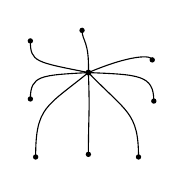
\begin{tikzpicture}[scale=.67,line cap=round]
\foreach \a/\b/\c/\d in {-1.1/.6/-1/.2,-1.1/-.5/-.9/-.05,-1/-1.6/-.8/-.65,0/-1.55/.03/-.8,.95/-1.6/.72/-.75,1.24/-.54/.95/-.04,1.21/.24/.8/.34,-.12/.80/.02/.60}{
\draw (0,0) .. controls (\c,\d) and (\a,\d) .. (\a,\b); \fill (\a,\b) circle(1.45pt);}
\fill (0,0) circle(1.6pt);
\end{tikzpicture}}

\[
\inserted{\mathrm{Aut}(G,\Gamma)\simeq}N(\Gamma)=\deleted{\unsure{\mathrm{Aut}(G,\Gamma)=|\mathrm{Aut}(G,T)=}}N(T)\deleted{=},\qquad N(\Gamma)/Z(\Gamma)=\mathrm{Aut}(G,\Gamma)\simeq\mathbb Z/2\mathbb Z
\]

\diagram{\begin{tikzcd}[ampersand replacement=\&,row sep=small]
\mathrm{Aut}\,\Gamma\\ 
\mathbb Z/2\mathbb Z\arrow[u,hook]
\end{tikzcd}}

\margin{\uline{NB} 1° et 3° sont les seuls cas abéliens}
\margin{\unsure{devant} $\longleftarrow$}

\uline{Corollaire} La donnée, sur un schéma $S$ de car. 0, d'une
forme $G$ de $\mathrm{GP}(1)$ et d'un sous-gpe étale fini $\Gamma$ de $G$,
cyclique d'ordre $n$ ($n\geq2$ donné), équivaut à celle d'une \unsure{Module dté|Module|Mod.}
\unsure{quadratique} \unsure{lisse} de rg 2 sur $S$.

% slanted
\margin{\unsure{expliciter} les foncteurs}

3) Soit $\Gamma=\mathbb D_2\inserted{=\mathbb Z_2\times\mathbb Z_2}$. Alors

\[
Z(\Gamma)=\Gamma
\]

$N(\Gamma)=\unsure{\mathfrak S_4|\mathscr S_4}$, $N(\Gamma)$ est l'unique ss-gpe de type
$\mathcal A_4$ qui contienne $\Gamma$, et $\Gamma\mapsto N=N(\Gamma)$,
$N\longmapsto\Gamma={}$ unique ss-gpe de type $\mathbb D_{2}$ de
$N$ $={}$ unique ss-gpe invariant ``\deleted{propre}'' \deleted{de}
de $N$ distinct de $[N,N]$ i.e. d'indice
$\ne2$ [ou encore d'indice 6], sont des
corr. 1-1 entre l'ens des sous-gpes
de $G$ de type $\mathbb D_2$, et l'ens des ss-gpes de type $\mathfrak S_4$.

\figure{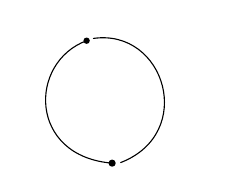
\begin{tikzpicture}[scale=.72,line cap=round]
\draw (-.35,1.08) .. controls (-1.38,.7) and (-1.38,-.96) .. (.10,-1.08);
\draw (.25,-1.07) .. controls (1.59,-.55) and (1.03,1.30) .. (-.23,1.12);
\fill (-.35,1.08) circle(1.6pt);\fill (.10,-1.08) circle(1.8pt);
\end{tikzpicture}}

\margin{\uline{NB} Ici $N(\Gamma)\to\mathrm{Aut}(\Gamma)$ non injectif (c'est le seul cas, avec le cas}

\[
N(\Gamma)/Z(\Gamma)\ \mathrel{\overset{\sim}{\rule{1.5em}{.4pt}}}\ \mathrm{Aut}(\Gamma)\simeq\mathfrak S_3
\]

\uline{Corollaire} La donnée d'un ss-groupe

\uline{Corollaire} \inserted{Sur base $S$ de car. 0,} la donnée d'un $(G,\Gamma)$, $G$ forme
de $\mathrm{GP}(1)$, \deleted{\unsure{$\Gamma\subset D_2$}} $\Gamma\subset G$ forme de $\mathbb D_2$, équivaut
à celle de $(G,\widetilde\Gamma)$, $G\ldots$, $\widetilde\Gamma\subset G$ forme de
$\mathfrak S_4$, ou encore à celle d'un torseur
sous $\mathfrak S_4$, ou encore d'un rev. étale de
degré 4 de $S$, ou celle d'un \uline{tétraèdre} sur $S$.

\margin{ou celle de \uline{octaèdre} \uline{\unsure{Orienté|Orientés}} sur $S$.}

% archive sheet number: 34
